% Provenance (never printed): see sources/outline_sources.md (Year 2: monsoons; El Niño--Southern
% Oscillation; the North Atlantic Oscillation; ocean--atmosphere coupling). Definitions after the
% IPCC AR6 glossary, the NOAA CPC ENSO FAQ and NAO pages, the NWS glossary and the IMD monsoon
% FAQ; indices from the CPC data files (data/derived/bachelor-2-{oni,oni-table,roni,nino34,nao});
% figures from figdata/bachelor-2/climvar.py; values of the examples, exercises and problem
% computed in the Book 4 scratch calculator calc/ch23.py.
\chapter{Variabilitas Iklim}\label{ch:b2:climate-variability}

Pada September 2026 permukaan laut di Pasifik ekuatorial tengah rata-rata bersuhu \qty{29.27}{\celsius},
padahal nilai September yang biasa adalah \qty{26.71}{\celsius}; lebih ke timur, sebagian samudra
lebih hangat lebih dari \qty{4}{\celsius} daripada biasanya, dan para prakirawan menilai peluangnya
lebih dari empat banding lima bahwa peristiwa itu, sebelum akhir tahun, melampaui setiap El~Niño sejak 1950. Peristiwa
rekor sebelumnya, pada 1982, 1997, dan 2015, memutihkan dan mematikan karang, membakar hutan tropis,
dan mendatangkan gelombang panas; tangkapan ikan teri Peru turun tajam bila air hangat itu bertahan. Samudra
dan atmosfer Pasifik tropis telah berayun, seperti yang terjadi setiap beberapa tahun, dan
ayunan itu menjangkau jauh melampaui Pasifik. Bab
ini menjelaskan ayunan-ayunan iklim semacam itu, yaitu \omterm{def:b2:climate-variability:monsoon}{monsun}, El~Niño dan La~Niña, \omterm{def:b2:climate-variability:nao}{Osilasi Atlantik
Utara}, serta apa yang menjadikan samudra sebagai ingatannya.
% ledger: data:b4-nino34, cpc:edd-2026-10, thirumalai24:bjerknes, cheung26:peru

\begin{recall}
\textbf{Dari volume-volume sekolah}: cuaca dan iklim; anomali suhu; lapisan campuran,
termoklin, dan upwelling; umpan balik iklim. \textbf{Dari volume Tahun 1}: sel
Hadley, angin pasat, zona konvergensi intertropis dan migrasi musimannya, sirkulasi
Walker, upwelling pantai. \textbf{Dari \cref{ch:b2:weather-systems}}: arus jet,
\omterm{def:b2:weather-systems:rossby}{gelombang Rossby}, \omterm{def:b2:weather-systems:cyclones}{siklon ekstratropis}, dan pemblokiran. \textbf{Dari buku-buku fisika}: kapasitas kalor
dan hukum pertama termodinamika.
\end{recall}

\section{Variabilitas dan ukuran-ukurannya}\label{sec:b2:climate-variability:measures}

Cuaca berubah dari hari ke hari; iklim, yaitu statistik cuaca, juga berubah, dari satu musim
atau satu tahun ke tahun berikutnya, bahkan ketika tidak ada yang berubah di luar sistem iklim. Sebagian
variabilitas itu berupa derau, tetapi sebagian besar tersusun dalam beberapa pola yang berulang, dengan
geografi dan skala waktunya sendiri.

\begin{definition}[Mode variabilitas iklim; indeks iklim; klimatologi]\label{def:b2:climate-variability:modes}
Yang disebut \emph{mode variabilitas iklim}\index{mode variabilitas iklim} adalah pola berulang dari
variabilitas alami sistem iklim, dengan pola spasial, musim, dan skala waktunya
sendiri, yang timbul dari dinamika atmosfer atau dari kopling antara samudra dan
atmosfer. Yang disebut \emph{indeks iklim}\index{indeks iklim} adalah deret waktu yang dibangun dari variabel-variabel
iklim dan meringkas keadaan pola semacam itu, misalnya selisih tekanan permukaan laut
antara Islandia dan Azores. Yang disebut \emph{klimatologi}\index{klimatologi} suatu variabel
adalah rata-ratanya selama suatu periode acuan, yang dihitung untuk setiap bulan kalender atau musim; periode
acuan baku panjangnya 30 tahun, saat ini 1991--2020.
\end{definition}
% ledger: ipccgl:modes, ipccgl:index, wmo:normal-30yr

Banyak mode digerakkan oleh proses-proses di dalam sistem iklim: mode itu merupakan bagian dari
variabilitas internalnya. Karena berulang dengan skala waktunya sendiri, mode itu menjadi sumber
keterprakiraan di luar jangkauan prakiraan cuaca, dari pekan sampai dekade. Indeks membuatnya
dapat diukur. Suatu indeks dihitung dari anomali, seperti dalam volume-volume sekolah, lalu
dihaluskan.
% ledger: ipccgl:modes

\begin{method}[Dari pengamatan ke indeks]\label{met:b2:climate-variability:index}
\begin{enumerate}
  \item Hitung \omterm{def:b2:climate-variability:modes}{klimatologi}: rata-rata variabel untuk setiap bulan kalender selama periode
        acuan.
  \item Kurangkan: anomali setiap bulan adalah nilainya dikurangi \omterm{def:b2:climate-variability:modes}{klimatologi} bulan itu.
        Siklus musiman hilang; yang tersisa adalah variabilitasnya.
  \item Haluskan anomali dengan rata-rata bergerak, yaitu rata-rata $n$ nilai berturutan yang berpusat pada
        setiap bulan, untuk menghilangkan fluktuasi yang lebih singkat daripada pola yang dikaji.
  \item Jika indeks itu akan dibandingkan dengan indeks lain, bagilah dengan simpangan bakunya: indeks
        itu lalu terbakukan, dalam satuan simpangan baku.
\end{enumerate}
\end{method}

\begin{example}[Sebuah anomali]\label{ex:b2:climate-variability:anomaly}
Suhu permukaan laut rata-rata Pasifik ekuatorial tengah antara \ang{5} LU dan
\ang{5} LS, \ang{170} BB dan \ang{120} BB adalah \qty{29.27}{\celsius} pada September 2026. \omterm{def:b2:climate-variability:modes}{Klimatologi}
Septembernya adalah \qty{26.71}{\celsius}, sehingga anomalinya $29.27 - 26.71 = \qty{2.56}{\celsius}$.
Pada September 1997 samudra yang sama bersuhu \qty{28.79}{\celsius} terhadap \qty{26.73}{\celsius}, suatu
anomali sebesar \qty{2.06}{\celsius}. Kedua \omterm{def:b2:climate-variability:modes}{klimatologi} itu sedikit berbeda karena periode acuannya
digeser setiap lima tahun: samudra itu sendiri telah menghangat.
% ledger: data:b4-nino34, cpc:oni-def
\end{example}

\section{Monsun}\label{sec:b2:climate-variability:monsoons}

\begin{definition}[Monsun]\label{def:b2:climate-variability:monsoon}
Yang disebut \emph{monsun}\index{monsun} adalah angin yang digerakkan secara termal, yang timbul dari pemanasan yang berbeda antara
suatu daratan dan samudra di dekatnya, dan yang membalik arahnya mengikuti musim, bersama
pembalikan musiman curah hujan yang dibawanya.
\end{definition}
% ledger: nws4:monsoon, ipccgl:monsoon

Di daratan, kalor Matahari musim panas tetap berada dalam lapisan tipis dekat permukaan, sedangkan laut mencampur
kalor yang sama ke bawah melalui lapisan campurannya, sedalam puluhan meter, dan jauh kurang menghangat. Udara di atas
daratan lebih menghangat, tekanannya di permukaan turun, dan udara lembap mengalir masuk dari laut, naik, mendingin, dan
menjadi hujan; di atas, udara kembali ke arah laut. Pada musim dingin daratan menjadi permukaan yang lebih dingin dan sirkulasinya
membalik. Secara keseluruhan, \omterm{def:b2:climate-variability:monsoon}{monsun-monsun} di planet ini membentuk satu pola global yang mendominasi siklus
tahunan hujan tropis dan subtropis; wilayahnya didefinisikan sebagai daerah-daerah tempat hujan rata-rata
musim panas setempat melebihi hujan musim dinginnya lebih dari \qty{2.5}{mm} sehari.
% ledger: nws4:monsoon, ipccgl:monsoon

\begin{omfigure}
\centering
\begin{tikzpicture}[font=\scriptsize, >=Stealth]
\foreach \col/\title in {0/{a\enspace musim panas}, 7.2/{b\enspace musim dingin}} {
  \begin{scope}[shift={(\col,0)}]
  \node[anchor=south west] at (0,3.0) {\textbf{\title}};
  \fill[ocBlue!18] (0,0) rectangle (3,0.35);
  \fill[brown!35] (3,0) -- (6.4,0) -- (6.4,0.5) -- (3,0.35) -- cycle;
  \node at (1.5,0.17) {laut};
  \node at (4.7,0.2) {darat};
  \end{scope}
}
% summer: low over the land, inflow from the sea, rising air and rain
\node[font=\small\bfseries, ocBlue] at (0.45,0.62) {H};
\node[font=\small\bfseries, ocRed] at (4.8,0.78) {L};
\node[ocRed, anchor=west] at (5.35,0.78) {panas};
\draw[->, thick] (1.0,0.98) -- (4.2,1.02);
\node at (2.4,0.66) {udara lembap dari laut};
\draw[->, thick] (4.8,1.15) -- (4.8,2.55);
\draw[->, thick] (4.45,2.8) -- (1.75,2.8);
\draw[->, thick] (1.4,2.6) -- (1.4,1.25);
\fill[black!15, draw=black!40] (4.0,1.9) .. controls (4.0,2.55) and (5.6,2.55) .. (5.6,1.9) -- cycle;
\foreach \x in {4.25,4.5,5.1,5.35} {\draw[ocBlue, dashed] (\x,1.85) -- (\x-0.1,1.2);}
\node[anchor=west] at (5.65,2.1) {hujan};
% winter: high over the land, dry outflow to the sea
\begin{scope}[shift={(7.2,0)}]
\node[font=\small\bfseries, ocRed] at (0.45,0.62) {L};
\node[font=\small\bfseries, ocBlue] at (4.8,0.78) {H};
\node[ocBlue, anchor=west] at (5.35,0.78) {dingin};
\draw[->, thick] (4.2,1.02) -- (1.0,0.98);
\node at (2.4,0.66) {udara kering dari darat};
\draw[->, thick] (1.4,1.25) -- (1.4,2.6);
\draw[->, thick] (1.75,2.8) -- (4.45,2.8);
\draw[->, thick] (4.8,2.55) -- (4.8,1.15);
\end{scope}
\end{tikzpicture}
\par\smallskip{\small \omterm{def:b2:climate-variability:monsoon}{Monsun} sebagai sirkulasi darat--laut (penampang skematis, tidak menurut skala): pada
musim panas daratan adalah permukaan yang lebih hangat, dengan tekanan rendah di permukaan tanah, aliran masuk udara lembap dari
laut, udara yang naik, dan hujan; pada musim dingin sirkulasinya membalik dan angin darat bersifat kering.}
\end{omfigure}
% ledger: nws4:monsoon, imd:heat-low

\omterm{def:b2:climate-variability:monsoon}{Monsun} Asia Selatan dan Asia Tenggara dimulai pada akhir Mei atau awal Juni, bergerak
ke arah timur laut, dan berakhir pada akhir September atau awal Oktober. Sebelumnya, daratan di sekitar
Laut Arab memanas: pada bulan Juni permukaan mengirimkan sekitar \qty{160}{W/m^2} kalor ke udara di atas
barat laut India yang gersang, Pakistan, dan Timur Tengah, dan di sana terbentuk depresi termal yang dangkal,
yang hanya mencapai sekitar \qty{1.5}{km}, dengan sedikit hujan; depresi termal yang lemah, seperti pada tahun kekeringan
1987, berarti tarikan yang lemah pada udara lembap dari samudra. Dari depresi itu, sebuah palung tekanan rendah yang memanjang, yaitu palung
\omterm{def:b2:climate-variability:monsoon}{monsun}, membentang sampai ujung Teluk Benggala; osilasi utara--selatannya mendatangkan periode
aktif dan jeda selama musim itu. Untuk India secara keseluruhan, hujan Juni sampai September rata-rata
\qty{88}{cm}, dengan simpangan baku \qty{9}{cm}, sekitar \qty{10}{\percent}: musim yang berada dalam
\qty{10}{\percent} dari rata-rata jangka panjang disebut normal. Di pesisir Kerala, tempat
badan cuaca nasional menyatakan awal \omterm{def:b2:climate-variability:monsoon}{monsun} berdasarkan curah hujan di empat belas stasiun,
angin, dan radiasi inframerah keluar yang diukur satelit, curah hujan rata-rata adalah
\qty{556}{mm} pada Juni dan \qty{659}{mm} pada Juli.
% ledger: ipccgl:monsoon, imd:heat-low, imd:lpa, imd:onset

\omterm{def:b2:climate-variability:monsoon}{Monsun} Afrika Barat membawa angin barat daya yang lembap dari Teluk Guinea, yang bergerak
ke utara dari Mei sampai September; hujannya mencapai puncak dekat \ang{12} LU pada akhir Agustus dan September lalu
mundur sejak Oktober.
% ledger: ipccgl:monsoon

Suatu \omterm{def:b2:climate-variability:monsoon}{monsun} teratur dalam waktunya, tetapi tidak teratur dalam jumlahnya, dan ayunan dari tahun ke tahun di
Pasifik tropis termasuk penyebabnya. Pada tahun-tahun El~Niño, India cenderung kekurangan hujan:
kekeringan tahun 1904, 1972, dan 1987 datang bersama El~Niño. Hubungan itu tidak pasti: pada 1997 sebuah
El~Niño yang kuat bertepatan dengan fase positif Dipol Samudra Hindia, sebuah mode yang dibahas di bawah, dan India
mengalami \omterm{def:b2:climate-variability:monsoon}{monsun} yang hampir normal.
% ledger: narang24:enso-monsoon, ipccgl:other-modes

\section{El Niño dan Osilasi Selatan}\label{sec:b2:climate-variability:enso}

Volume Tahun~1 telah menjelaskan sirkulasi Walker: udara naik di atas Pasifik barat yang hangat,
mengalir ke timur di lapisan atas, turun di atas Pasifik timur yang sejuk, dan kembali ke barat bersama angin
pasat. Di samudra di bawahnya, angin pasat menumpuk air hangat di barat, tempat termoklin
dalam, dan menarik air dingin ke atas di sepanjang khatulistiwa di timur, tempat termoklin dangkal. Keadaan ini tidak
tetap.

\begin{definition}[El Niño--Osilasi Selatan; El Niño; La Niña; Osilasi Selatan]\label{def:b2:climate-variability:enso}
Yang disebut \emph{El Niño--Osilasi Selatan}\index{El Niño--Osilasi Selatan} (ENSO) adalah
mode terkopel samudra--atmosfer di Pasifik tropis: variasi koheren dari tahun ke tahun pada
suhu permukaan laut, curah hujan konvektif, tekanan permukaan, dan sirkulasi di sepanjang
Pasifik ekuatorial, dengan skala waktu yang disukai dua sampai sekitar tujuh tahun. \emph{El
Niño}\index{El Niño} adalah fase hangatnya, yaitu penghangatan permukaan laut di Pasifik ekuatorial tengah dan
timur-tengah; \emph{La Niña}\index{La Niña} adalah fase dinginnya, yaitu pendinginan di
wilayah yang sama. Yang disebut \emph{Osilasi Selatan}\index{Osilasi Selatan} adalah bagian atmosferiknya,
yaitu jungkat-jungkit tekanan permukaan antara Pasifik tropis barat dan timur: selama El~Niño
tekanan lebih tinggi daripada rata-rata di atas Indonesia dan Pasifik barat dan lebih rendah di atas
Pasifik timur, dan sebaliknya selama La~Niña.
\end{definition}
% ledger: cpc:enso-faq, cpc:enso-faq-so, ipccgl:enso

Selama El~Niño, angin pasat timuran melemah di sepanjang khatulistiwa, dan di barat
angin lapisan bawah bahkan dapat bertiup dari barat; air hangat dari barat menyebar ke timur, dan
konveksi dalam beserta hujannya mengikutinya, sehingga Indonesia dan Australia utara menjadi lebih kering. Permukaan laut
Pasifik timur-tengah biasanya \qtyrange{1.5}{2.5}{\celsius} lebih hangat daripada rata-rata, dan
termoklin di sana terletak pada \qtyrange{150}{175}{m}, lebih dalam daripada biasanya. Selama La~Niña angin
pasat menguat di seluruh cekungan, permukaan laut \qtyrange{1}{2}{\celsius} lebih dingin daripada
rata-rata, dan termoklin di timur naik ke \qtyrange{50}{100}{m}. Sirkulasi Walker
melemah selama El~Niño dan menguat selama La~Niña. Episode-episodenya biasanya berulang setiap tiga sampai
lima tahun, dengan selang yang berkisar antara dua dan tujuh tahun; El~Niño biasanya berlangsung sembilan sampai
dua belas bulan, La~Niña satu sampai tiga tahun. Keduanya cenderung berkembang antara Maret dan Juni,
mencapai puncak antara Desember dan April, dan melemah antara Mei dan Juli; dampaknya paling kuat
dari Desember sampai April, ketika permukaan laut ekuatorial paling hangat.
% ledger: cpc:enso-faq-features, cpc:enso-faq-timing

\begin{omfigure}
\centering
\begin{tikzpicture}[font=\scriptsize, >=Stealth, x=1cm, y=0.8cm]
\foreach \row/\title/\tw/\te/\rx/\cwidth in {
    0/{a\enspace netral}/1.15/0.35/1.6/1.0,
    -4.6/{b\enspace El Niño}/0.95/0.85/5.6/1.4,
    -9.2/{c\enspace La Niña}/1.3/0.18/1.0/0.8} {
  \begin{scope}[shift={(0,\row)}]
  \node[anchor=south west] at (0,2.55) {\textbf{\title}};
  % ocean: warm layer above the thermocline
  \fill[ocBlue!20] (0,-1.5) rectangle (11,0);
  \fill[omWarm!25] (0,0) -- (0,-\tw) .. controls (4,-\tw) and (7,-\te) .. (11,-\te) -- (11,0) -- cycle;
  \draw[thick, ocBlue!70!black] (0,-\tw) .. controls (4,-\tw) and (7,-\te) .. (11,-\te);
  \draw (0,0) -- (11,0);
  % convection and Walker cell
  \fill[black!15, draw=black!40] ({\rx-\cwidth/2},0.5) .. controls ({\rx-\cwidth/2},2.1) and ({\rx+\cwidth/2},2.1) .. ({\rx+\cwidth/2},0.5) -- cycle;
  \draw[->, thick] (\rx,0.55) -- (\rx,2.15);
  \draw[->, thick] ({\rx+0.4},2.3) -- (9.6,2.3);
  \draw[->, thick] (10.0,2.1) -- (10.0,0.5);
  \draw[->, thick] (9.6,0.3) -- ({\rx+0.7},0.3);
  \end{scope}
}
\node[anchor=west] at (2.3,1.4) {udara naik, hujan};
\node[anchor=east] at (9.9,1.4) {udara turun};
\node at (6.0,0.55) {angin pasat};
\node[anchor=west, ocBlue!70!black] at (7.6,-0.95) {termoklin};
\node[anchor=east] at (4.8,-4.6+1.4) {hujan bergeser ke timur};
\node at (8.2,-4.6+0.55) {angin pasat lemah};
\node at (6.0,-9.2+0.55) {angin pasat kuat};
\node[ocBlue!70!black, align=center] at (9.6,-9.2-0.8) {air dingin\\dekat permukaan};
\node[anchor=north west] at (0,-9.2-1.55) {barat (Indonesia)};
\node[anchor=north east] at (11,-9.2-1.55) {timur (Amerika Selatan)};
\end{tikzpicture}
\par\smallskip{\small Pasifik ekuatorial di sepanjang khatulistiwa dalam tiga fase ENSO
(skematis, tidak menurut skala): sirkulasi Walker di atas, lapisan atas yang hangat dan
termoklin di bawah. Selama El~Niño angin pasat melemah, air hangat dan hujan menyebar ke timur,
dan termoklin di timur mendalam sampai \qtyrange{150}{175}{m}; selama La~Niña angin pasat
menguat dan termoklin di timur naik ke \qtyrange{50}{100}{m}.}
\end{omfigure}
% ledger: cpc:enso-faq-features, climategov:walker

Nama-nama itu berasal dari abad yang berbeda dan ilmu yang berbeda. Para nelayan di pesisir
Amerika Selatan memperhatikan penghangatan perairan pantai mereka sekitar Natal yang mengganggu
perikanan, dan menyebutnya El~Niño, sang anak laki-laki. Sir Gilbert Walker menemukan \omterm{def:b2:climate-variability:enso}{Osilasi
Selatan} di atmosfer, tanpa mengaitkannya dengan samudra. Baru pada akhir 1960-an Jacob Bjerknes dan kawan-kawan menyadari bahwa
keduanya adalah satu fenomena. Istilah La~Niña dan netral mulai menonjol pada 1980-an.
% ledger: climategov:enso-history, ipccgl:enso

\begin{history}[Anak laki-laki para nelayan]
\begin{minipage}[t]{0.54\linewidth}\vspace{0pt}
Di lepas pesisir Peru yang kering, air dingin yang ditarik angin ke atas di sepanjang pantai kaya akan
nutrien dan menghidupi perikanan yang produktif. Para nelayannya mengenal penghangatan yang datang sekitar
Natal, ketika ikan menjadi langka, dan menamainya dengan nama sang anak dari musim itu. Tangkapan
ikan teri Peru masih mengikuti ENSO: dalam sebuah analisis baru-baru ini, anomali suhu tinggi yang
berkepanjangan membuat tangkapan yang sangat rendah lebih dari sembilan kali lebih mungkin, dengan penurunan median
tangkapan sekitar \qty{60}{\percent}; El~Niño kuat tahun 1997--98 menonjol dalam catatan itu.
\end{minipage}\hfill
\begin{minipage}[t]{0.42\linewidth}\vspace{0pt}
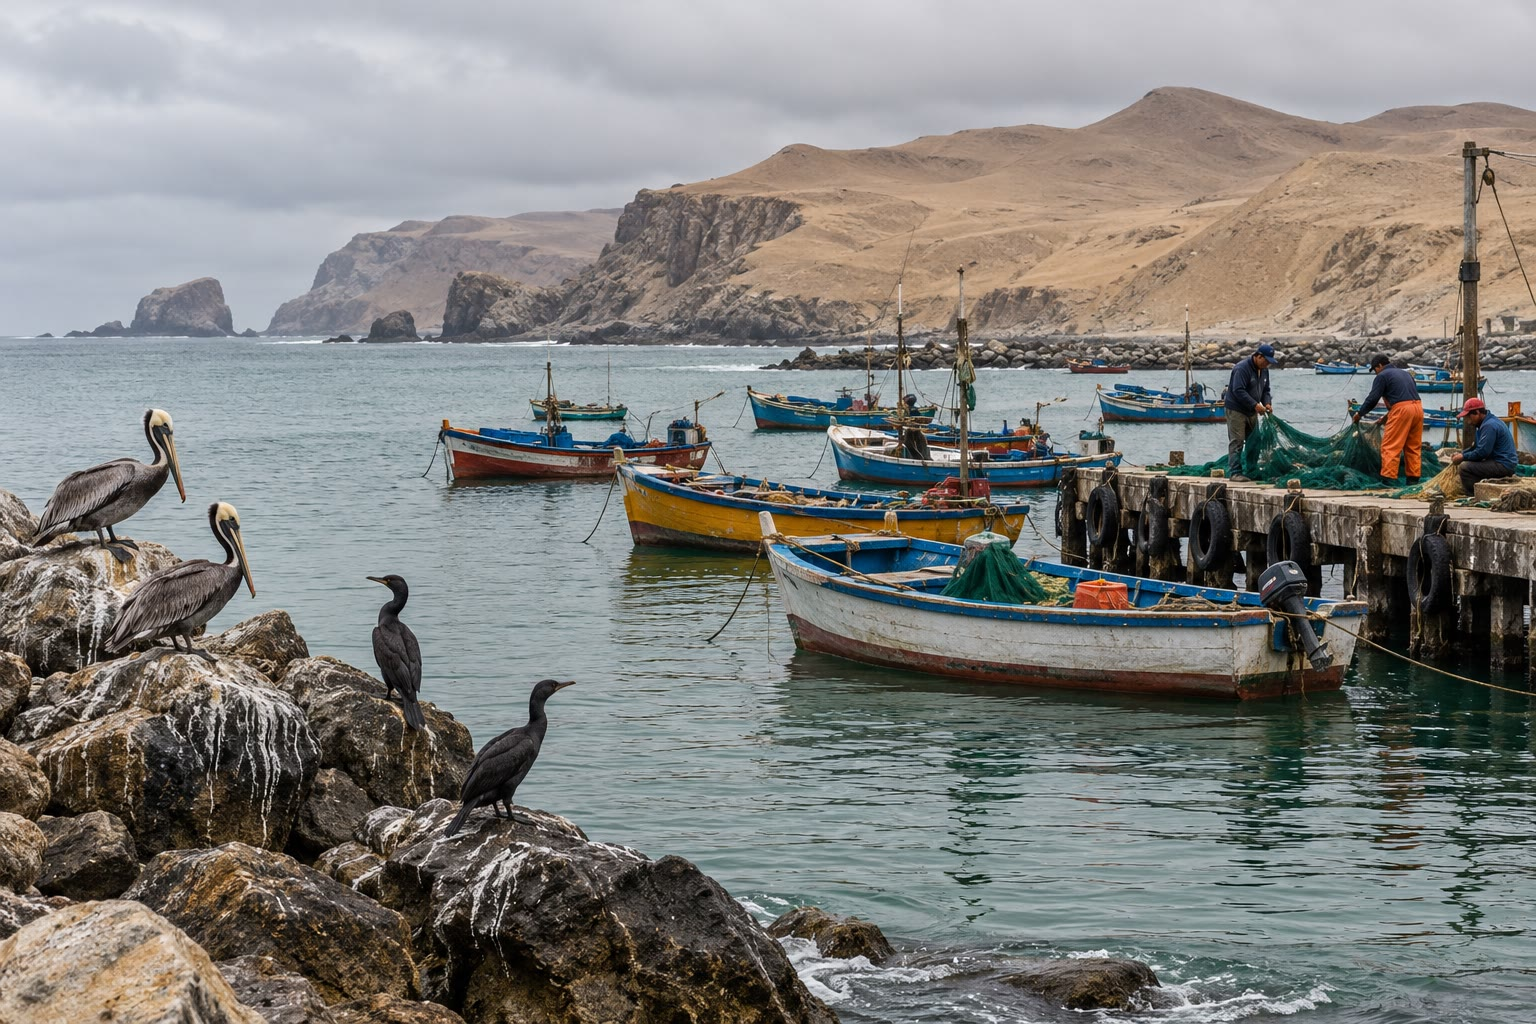
\includegraphics[width=\linewidth]{images/book4/ai/b2-fishing-harbour.jpg}

{\scriptsize Perahu-perahu nelayan di pelabuhan di pesisir gurun dengan air upwelling yang dingin
(ilustrasi buatan AI).}
\end{minipage}
% ledger: climategov:enso-history, cheung26:peru, stewart:upwelling
\end{history}

Mengapa sistem itu berayun sama sekali? Karena samudra dan atmosfer Pasifik ekuatorial
saling memperkuat anomali masing-masing.

\begin{definition}[Umpan balik Bjerknes]\label{def:b2:climate-variability:bjerknes}
Yang disebut \emph{umpan balik Bjerknes}\index{umpan balik Bjerknes} adalah umpan balik positif antara
suhu permukaan laut, angin, dan arus laut di Pasifik ekuatorial: penghangatan di
timur melemahkan kontras suhu dan tekanan timur--barat, sehingga melemahkan angin pasat;
angin pasat yang lebih lemah membiarkan air hangat dari barat menyebar ke timur dan mengangkat lebih sedikit air dingin di
timur, yang menghangatkan timur lebih jauh. Lingkar yang sama memperkuat pendinginan.
\end{definition}
% ledger: thirumalai24:bjerknes, cpc:enso-faq-timing

\begin{omfigure}
\centering
\begin{tikzpicture}[font=\small, >=Stealth, box/.style={draw, rounded corners=2pt, fill=omDef!8,
  align=center, text width=4.3cm, minimum height=1.05cm, inner sep=3pt}]
\node[box] (a) at (0,2) {Pasifik ekuatorial timur\\lebih hangat daripada biasa};
\node[box] (b) at (6.2,2) {kontras suhu dan tekanan\\timur--barat lebih kecil};
\node[box] (c) at (6.2,0) {angin pasat lebih lemah};
\node[box] (d) at (0,0) {air hangat meluas ke timur,\\lebih sedikit air dingin naik};
\draw[->, very thick, ocRed] (a) -- (b);
\draw[->, very thick, ocRed] (b) -- (c);
\draw[->, very thick, ocRed] (c) -- (d);
\draw[->, very thick, ocRed] (d) -- (a);
\node[ocRed, font=\bfseries] at (3.1,1) {$+$};
\end{tikzpicture}
\par\smallskip{\small \omterm{def:b2:climate-variability:bjerknes}{Umpan balik Bjerknes}, digambar untuk penghangatan; dengan setiap panah dibalik,
lingkar yang sama memperdalam pendinginan. Lingkar positif semacam ini memperkuat gangguan kecil.}
\end{omfigure}
% ledger: thirumalai24:bjerknes

Umpan balik positif menjelaskan bagaimana suatu anomali tumbuh, bukan bagaimana ia dimulai atau berakhir. Menurut salah satu penjelasan masa kini,
El~Niño dimulai ketika fluktuasi acak angin pasat melemahkan arus-arus ekuatorial yang
menahan air hangat di barat; kolam hangat menyebar ke timur, konveksi mengikutinya,
\omterm{def:b2:climate-variability:bjerknes}{umpan balik Bjerknes} mengambil alih, dan peristiwa itu tumbuh. Peristiwa La~Niña, menurut penjelasan yang sama,
dipicu oleh El~Niño yang mendahuluinya. Model-model paling sederhana yang membuat sistem itu berosilasi, termasuk osilator
pengisian ulang, mengopel dua besaran: anomali suhu permukaan laut di Pasifik
tengah dan volume air lapisan atas yang hangat yang tersimpan di sepanjang khatulistiwa. Anomali
suhu menguras atau mengisi kembali simpanan itu melalui angin yang digerakkannya, dan simpanan itu, melalui
kedalaman termoklin, menyiapkan fase berikutnya. \Cref{exo:b2:climate-variability:10} menyelesaikan
sepasang persamaan semacam itu.
% ledger: thirumalai24:bjerknes, stuecker25:ro

Untuk mengikuti ENSO, pusat-pusat pemantauan memakai indeks.

\begin{definition}[Indeks Niño-3.4; Indeks Niño Oseanik]\label{def:b2:climate-variability:oni}
Yang disebut \emph{indeks Niño-3.4}\index{indeks Niño-3.4} adalah anomali bulanan suhu permukaan
laut yang dirata-ratakan atas wilayah \ang{5} LU--\ang{5} LS, \ang{170} BB--\ang{120} BB, relatif terhadap
\omterm{def:b2:climate-variability:modes}{klimatologi} suatu periode dasar 30 tahun yang berpusat pada tahun itu, yang diperbarui setiap lima tahun. Yang disebut
\emph{Indeks Niño Oseanik}\index{Indeks Niño Oseanik} (ONI) adalah rata-rata bergerak tiga bulanannya. Suatu
episode El~Niño (La~Niña) adalah deretan sedikitnya lima musim tiga bulanan bertumpang tindih yang berturutan
dengan ONI sama dengan atau di atas \qty{+0.5}{\celsius} (sama dengan atau di bawah \qty{-0.5}{\celsius}).
\end{definition}
% ledger: cpc:oni-def, cpc:enso-faq

Musim-musim itu bertumpang tindih: DJF, JFM, FMA, dan seterusnya, masing-masing rata-rata tiga bulan, masing-masing berbagi dua
bulan dengan musim berikutnya. Indeks kedua, Indeks \omterm{def:b2:climate-variability:enso}{Osilasi Selatan}, mengikuti atmosfer: indeks ini
dihitung dari simpangan selisih tekanan antara Tahiti dan Darwin, yang negatif
selama El~Niño dan positif selama La~Niña. Sejak Februari 2026 indeks resmi untuk memantau
ENSO adalah ONI relatif, yang dihitung dari anomali Niño-3.4 dikurangi anomali rata-rata seluruh
samudra tropis antara \ang{20} LU dan \ang{20} LS, lalu diskalakan ulang ke amplitudo ONI. Karena
diukur terhadap seluruh daerah tropis, indeks ini kurang bergantung pada pilihan periode dasar selama samudra
menghangat, dan lebih erat kaitannya dengan curah hujan Pasifik tropis. Pada September 2026
anomali relatif wilayah Niño-3.4 adalah \qty{2.08}{\celsius}, dibandingkan dengan \qty{2.56}{\celsius}
pada \cref{ex:b2:climate-variability:anomaly}: sekitar setengah derajat dari anomali tradisional itu adalah
kehangatan samudra tropis secara keseluruhan.
% ledger: cpc:enso-faq-so, pns:roni, data:b4-rnino34

\begin{omfigure}
\centering
% figdata/bachelor-2/climvar.py part oni
\begin{tikzpicture}
\begin{axis}[width=\linewidth, height=6.0cm, xmin=1950, xmax=2027, ymin=-2.4, ymax=3.0,
  xlabel={tahun}, ylabel={indeks (\unit{\celsius})}, tick label style={font=\scriptsize},
  label style={font=\small}, xtick={1950,1960,...,2020}, x tick label style={/pgf/number
  format/1000 sep={}}, legend style={font=\scriptsize, at={(0.5,1.02)}, anchor=south,
  draw=none, legend columns=3, /tikz/every even column/.append style={column sep=6pt}},
  legend cell align=left]
\addplot[fill=ocRed!70, draw=none, area legend] table[x=t, y=pos]
  {figdata/out/bachelor-2-climvar-oni.dat} \closedcycle;
\addlegendentry{ONI, sisi El Niño}
\addplot[fill=ocBlue!70, draw=none, area legend] table[x=t, y=neg]
  {figdata/out/bachelor-2-climvar-oni.dat} \closedcycle;
\addlegendentry{ONI, sisi La Niña}
\addplot[black, thin] table[x=t, y=roni] {figdata/out/bachelor-2-climvar-oni.dat};
\addlegendentry{ONI relatif}
\addplot[black!60, densely dashed, domain=1950:2027, samples=2] {0.5};
\addplot[black!60, densely dashed, domain=1950:2027, samples=2] {-0.5};
\end{axis}
\end{tikzpicture}
\par\smallskip{\small \omterm{def:b2:climate-variability:oni}{Indeks Niño Oseanik} dari DJF 1950 sampai JAS 2026 (satu nilai per
musim tiga bulanan, diplot pada bulan tengahnya), dan ONI relatif, indeks resmi sejak
Februari 2026; garis putus-putus: ambang $\pm\qty{0.5}{\celsius}$. Data: Pusat Prediksi Iklim
NOAA, sebagaimana diambil pada 23 Oktober 2026.}
\end{omfigure}
% ledger: data:b4-oni, data:b4-roni

Bila dihitung dengan aturan lima musim pada tabel Pusat Prediksi Iklim (CPC) NOAA, ONI menunjukkan 25
episode El~Niño dan 21 episode La~Niña antara 1950 dan musim panas 2026. Puncak El~Niño
terkuat adalah \qty{2.4}{\celsius} pada akhir 1997 dan \qty{2.6}{\celsius} pada akhir 2015. Kedua indeks itu
paling banyak berbeda dalam tahun-tahun terakhir: pada Juli--September 2026 ONI berada pada \qty{2.2}{\celsius} dan
indeks relatif pada \qty{1.7}{\celsius}.
% ledger: data:b4-oni, data:b4-roni

\begin{dated}{2026}
Dalam diskusinya tanggal 8 Oktober 2026 Pusat Prediksi Iklim mempertahankan peringatan El~Niño: anomali
Niño-3.4 relatif telah mencapai \qty{+2.1}{\celsius} pada September, sebagian Pasifik ekuatorial
timur lebih dari \qty{4}{\celsius} di atas rata-rata, air di kedalaman di timur
lebih dari \qty{10}{\celsius} di atasnya, dan indeks-indeks \omterm{def:b2:climate-variability:enso}{Osilasi Selatan} negatif secara
signifikan. El~Niño
yang kuat sampai sangat kuat dinilai mungkin berlangsung sampai Januari--Maret 2027, dan peluang bahwa
indeks relatif akan melampaui \qty{2.5}{\celsius}, melebihi setiap peristiwa sejak 1950, ditetapkan
\qty{83}{\percent} untuk Oktober--Desember.
% ledger: cpc:edd-2026-10, data:b4-rnino34
\end{dated}

\section{Osilasi Atlantik Utara dan telekoneksi}\label{sec:b2:climate-variability:nao}

\begin{definition}[Osilasi Atlantik Utara]\label{def:b2:climate-variability:nao}
Yang disebut \emph{Osilasi Atlantik Utara}\index{Osilasi Atlantik Utara} (NAO) adalah mode utama
variabilitas atmosfer di atas Atlantik Utara: jungkat-jungkit tekanan permukaan laut antara
Depresi Islandia dan Antisiklon Azores. Indeksnya positif bila keduanya lebih kuat daripada rata-rata, sehingga
selisih tekanan di antara keduanya besar, dan negatif bila keduanya lebih lemah.
\end{definition}
% ledger: ipccgl:other-modes, climategov:nao, cpc:nao-teledoc

NAO mengendalikan angin baratan dari bab sebelumnya. Dalam fase positifnya, selisih tekanan yang lebih besar
menggerakkan arus jet Atlantik yang lebih kuat dan menggeser jalur badai ke utara: Eropa utara
mengalami musim dingin yang lebih berbadai, lebih basah, dan lebih lunak, Eropa selatan musim dingin yang lebih kering, Amerika Utara bagian timur
lebih sedikit serbuan udara dingin, dan Greenland musim dingin yang lebih dingin. Fase negatif membalik anomali-anomali
itu. Pada akhir abad kedelapan belas seorang misionaris sudah mencatat bahwa musim dingin yang lunak di
Greenland datang bersama musim dingin yang keras di Denmark, dan sebaliknya.
% ledger: climategov:nao, cpc:nao-teledoc

NAO adalah salah satu pola atmosfer yang paling menonjol pada setiap musim, dan pola ini
berkorelasi kuat dengan mode lain, yaitu Osilasi Arktik. NAO juga bervariasi dalam skala dekade: fase negatif mendominasi
dari pertengahan 1950-an sampai musim dingin 1978--79, dan fase positif dari 1979--80 sampai 1994--95.
% ledger: cpc:nao-teledoc, climategov:nao

\begin{omfigure}
\centering
% figdata/bachelor-2/climvar.py part nao
\begin{tikzpicture}
\begin{axis}[width=\linewidth, height=5.4cm, xmin=1950, xmax=2027, ymin=-1.9, ymax=1.9,
  ytick={-1,0,1},
  xlabel={musim dingin (tahun bulan Januarinya)}, ylabel={indeks NAO (rata-rata DJF)},
  tick label style={font=\scriptsize}, label style={font=\small}, xtick={1950,1960,...,2020},
  x tick label style={/pgf/number format/1000 sep={}}, legend style={font=\scriptsize,
  at={(0.5,1.02)}, anchor=south, draw=none, legend columns=2,
  /tikz/every even column/.append style={column sep=6pt}},
  legend cell align=left, unbounded coords=jump]
\addplot[ybar, bar width=0.6, fill=omDef!55, draw=none, area legend] table[x=year, y=nao]
  {figdata/out/bachelor-2-climvar-nao.dat};
\addlegendentry{rata-rata musim dingin}
\addplot[ocRed, thick] table[x=year, y=run5] {figdata/out/bachelor-2-climvar-nao.dat};
\addlegendentry{rata-rata bergerak 5 musim dingin}
\end{axis}
\end{tikzpicture}
\par\smallskip{\small Rata-rata musim dingin (Desember--Februari) dari indeks NAO bulanan Pusat Prediksi
Iklim NOAA, 1951--2026, dalam satuan simpangan baku, dengan rata-rata bergerak lima musim dingin
yang berpusat. Musim dingin terendah adalah 2010 ($-1.67$), yang tertinggi 2015 ($+1.66$).}
\end{omfigure}
% ledger: data:b4-nao, cpc:nao-teledoc

NAO, ENSO, dan mode-mode lain bekerja jauh dari tempat mode itu diukur.

\begin{definition}[Telekoneksi]\label{def:b2:climate-variability:teleconnection}
Yang disebut \emph{telekoneksi}\index{telekoneksi} adalah keterkaitan antara variabel-variabel iklim di
tempat-tempat tetap yang berjauhan, yang dihubungkan oleh proses-proses fisis di sepanjang lintasan di atmosfer atau
samudra, seperti rangkaian \omterm{def:b2:weather-systems:rossby}{gelombang Rossby}, pergeseran arus jet dan jalur badai, atau perubahan
sirkulasi Walker.
\end{definition}
% ledger: ipccgl:teleconnection

Selama El~Niño curah hujan di daerah tropis berubah dari Indonesia sampai Amerika Selatan, sekitar separuh
keliling dunia, dan dari daerah tropis anomali-anomali itu merambat ke lintang tengah melalui lintasan-lintasan
dalam definisi itu; \omterm{def:b2:climate-variability:monsoon}{monsun} India dari subbab sebelumnya adalah salah satu ujungnya. Mode-mode lain
telah dinamai di setiap samudra: Dipol Samudra Hindia, yaitu jungkat-jungkit timur--barat suhu permukaan
laut di Samudra Hindia tropis yang fase positifnya mendinginkan laut di lepas Sumatra dan Jawa
dan menghangatkannya di lepas Somalia, yang berkembang pada musim panas belahan utara, matang pada musim gugur, dan mengubah
hujan di Australia, Asia Tenggara, dan Afrika Timur; Mode Annular Selatan, yaitu perubahan
kekuatan dan lintang sabuk angin baratan di sekitar Antarktika; dan variabilitas dekadal
Pasifik, yang lebih lambat daripada ENSO.
% ledger: cpc:enso-faq, ipccgl:other-modes, ipccgl:teleconnection, narang24:enso-monsoon

\section{Samudra sebagai ingatan}\label{sec:b2:climate-variability:memory}

\Cref{ch:b2:weather-systems} mendapati bahwa atmosfer melupakan cuacanya dalam sekitar dua pekan.
Anomali iklim yang bertahan semusim harus tersimpan di suatu tempat, dan simpanan yang jelas adalah lapisan
campuran samudra: lapisan campuran yang lebih dalam menyimpan lebih banyak kalor dan memiliki inersia termal yang lebih besar. Model paling sederhana memperlakukan
anomali itu sebagai reservoir yang membocorkan kalor ke atmosfer.
% ledger: shi22:memory

\begin{proposition}[Waktu redam anomali lapisan campuran]\label{prop:b2:climate-variability:damping}
Misalkan lapisan campuran dengan kedalaman $h$, massa jenis $\rho$, dan kalor jenis $c_p$ membawa anomali suhu
$T'$, dan misalkan permukaan kehilangan fluks kalor tambahan $\alpha T'$ per satuan luas ke atmosfer,
dengan $\alpha > 0$. Maka, tanpa gaya paksa lain,
\[
  T'(t) = T'(0)\,\mathrm{e}^{-t/\tau}, \qquad \tau = \frac{\rho\,c_p\,h}{\alpha} .
\]
\end{proposition}

\begin{proof}
Kandungan kalor anomali itu per satuan luas adalah $\rho c_p h T'$; hukum pertama memberikan $\rho c_p h
\,\mathrm{d}T'/\mathrm{d}t = -\alpha T'$, suatu persamaan linear yang penyelesaiannya adalah peluruhan
eksponensial dengan konstanta waktu $\tau$.
\end{proof}
% ledger: shi22:memory

\begin{example}[Ingatan samudra lintang tengah]\label{ex:b2:climate-variability:tau}
Di atas samudra lintang tengah, fluks kalor permukaan menanggapi anomali suhu permukaan laut
dengan $\alpha = \qty{16.1}{W.m^{-2}.K^{-1}}$ rata-rata. Untuk lapisan campuran
sedalam \qty{50}{m}, dengan $\rho = \qty{1025}{kg/m^3}$ dan $c_p = \qty{3992}{J.kg^{-1}.K^{-1}}$,
$\tau = 1025 \times 3992 \times 50/16.1 = \qty{1.27e7}{s} = \qty{147}{\day}$, hampir lima
bulan; lapisan sedalam \qty{100}{m} mengingat dua kali lebih lama.
\end{example}
% ledger: wang24:shff, noaa:seawater-1025, teos10:cp0

Anomali yang nyata juga dipaksa, setiap hari, oleh cuaca: fluks kalor acak yang, sendirian,
akan menghasilkan derau putih, tanpa ingatan dari satu bulan ke bulan berikutnya. Bila ditambahkan pada peredaman, fluks itu
memberikan persamaan $\mathrm{d}T'/\mathrm{d}t = -T'/\tau + F(t)$ dengan $F$ acak: samudra menjumlahkan
gaya paksa acak itu selama waktu berorde $\tau$ dan melupakannya setelah itu. Hasilnya disebut
derau merah. Korelasi jedanya, yaitu korelasi antara anomali dan dirinya sendiri beberapa waktu kemudian,
turun sebagai $\mathrm{e}^{-\text{jeda}/\tau}$ (diterima), dan variasi lambat di dalamnya jauh lebih kuat
daripada dalam gaya paksanya. Model stokastik ingatan samudra ini adalah acuan baku yang
menjadi pembanding untuk mengukur persistensi anomali nyata, suatu sumber keterprakiraan di luar
skala waktu cuaca; karena kedalaman lapisan campuran menentukan ingatan itu, pendangkalan
lapisan campuran yang diproyeksikan untuk abad ini berarti ingatan yang lebih pendek.
% ledger: shi22:memory

\begin{omfigure}
\centering
% figdata/bachelor-2/climvar.py parts rednoise, acf
\begin{tikzpicture}
\begin{groupplot}[group style={group size=2 by 1, horizontal sep=1.6cm},
  tick label style={font=\scriptsize}, label style={font=\small}]
\nextgroupplot[width=0.62\linewidth, height=5.0cm, xmin=0, xmax=360, ymin=-1.6, ymax=1.6,
  xlabel={bulan}, ylabel={anomali (\unit{K})}, xtick={0,60,...,360},
  legend style={font=\scriptsize, at={(0.5,1.02)}, anchor=south, draw=none, legend columns=2},
  legend cell align=left]
\addplot[black!45, thin] table[x=month, y=white] {figdata/out/bachelor-2-climvar-rednoise.dat};
\addlegendentry{derau putih}
\addplot[ocRed, thick] table[x=month, y=red] {figdata/out/bachelor-2-climvar-rednoise.dat};
\addlegendentry{derau merah, $\tau = \qty{147}{\day}$}
\nextgroupplot[width=0.36\linewidth, height=5.0cm, xmin=0, xmax=24, ymin=0, ymax=1.05,
  xlabel={jeda (bulan)}, ylabel={korelasi jeda}, xtick={0,6,...,24},
  legend style={font=\scriptsize, at={(0.98,0.98)}, anchor=north east, draw=none},
  legend cell align=left]
\addplot[black, densely dashed] table[x=lag_months, y=theory] {figdata/out/bachelor-2-climvar-acf.dat};
\addlegendentry{$\mathrm{e}^{-\text{jeda}/\tau}$}
\addplot[only marks, mark=*, mark size=1.1pt, ocRed] table[x=lag_months, y=sample]
  {figdata/out/bachelor-2-climvar-acf.dat};
\addlegendentry{simulasi}
\end{groupplot}
\end{tikzpicture}
\par\smallskip{\small Derau merah dan derau putih dengan simpangan baku yang sama, 0.5~K, sebagai
rata-rata bulanan selama 30 tahun (kiri): lapisan campuran pada
\cref{ex:b2:climate-variability:tau} mengubah gaya paksa harian yang acak menjadi ayunan lambat. Kanan: korelasi
jeda dari simulasi 2000 tahun dibandingkan dengan $\mathrm{e}^{-\text{jeda}/\tau}$.}
\end{omfigure}
% ledger: shi22:memory, wang24:shff

ENSO memerlukan lebih dari ingatan pasif ini. Anomalinya tidak hanya melibatkan lapisan campuran tetapi
seluruh lapisan hangat di atas termoklin, yang bergerak puluhan meter, dan angin yang digerakkan
anomali itu berbalik memengaruhi samudra melalui lingkar Bjerknes. Samudra menyediakan kelambatan,
atmosfer menyediakan kopling; tidak satu pun dari keduanya sendirian menghasilkan osilasi. Kelambatan itulah yang diandalkan
para prakirawan pada Oktober 2026 ketika mereka menilai El~Niño yang kuat kemungkinan bertahan sampai
Januari--Maret 2027.
% ledger: cpc:enso-faq-features, cpc:enso-faq-timing, climategov:enso-history, cpc:edd-2026-10

\section*{Latihan}\label{sec:b2:climate-variability:exercises}

Data untuk latihan, kecuali dinyatakan lain: air laut $\rho = \qty{1025}{kg/m^3}$ dan $c_p =
\qty{3992}{J.kg^{-1}.K^{-1}}$; udara $c_p = \qty{1004.5}{J.kg^{-1}.K^{-1}}$; $g =
\qty{9.81}{m.s^{-2}}$; koefisien peredaman fluks kalor permukaan $\alpha =
\qty{16.1}{W.m^{-2}.K^{-1}}$; satu bulan adalah $365.25/12 = 30.44$ hari.
% ledger: noaa:seawater-1025, teos10:cp0, wang24:shff

\begin{exercise}[$\star$]\label{exo:b2:climate-variability:1}
Di wilayah Niño-3.4 suhu permukaan laut rata-rata adalah \qty{29.27}{\celsius} pada September
2026 dan \qty{28.79}{\celsius} pada September 1997; \omterm{def:b2:climate-variability:modes}{klimatologi} yang dipakai untuk kedua bulan September itu
adalah \qty{26.71}{\celsius} dan \qty{26.73}{\celsius}. (a) Hitung kedua anomali itu. (b) September
mana yang lebih hangat, dan anomali mana yang lebih besar? (c) Mengapa \omterm{def:b2:climate-variability:modes}{klimatologinya} tidak sama untuk
kedua tahun itu?
\end{exercise}
% ledger: data:b4-nino34, cpc:oni-def

\begin{exercise}[$\star$]\label{exo:b2:climate-variability:2}
Anomali Niño-3.4 bulanan dari Juni sampai Desember 2023 adalah 0.79, 0.95, 1.28, 1.55, 1.68, 2.01,
dan \qty{2.02}{\celsius}. (a) Hitung ONI musim JJA sampai OND. (b) Tabel
Pusat Prediksi Iklim memberikan 1.0, 1.3, 1.5, 1.7, dan 1.9. Bandingkan. (c) Pada musim apa
ONI pertama kali mencapai ambang peristiwa kuat, \qty{1.5}{\celsius}?
\end{exercise}
% ledger: data:b4-nino34-2023, data:b4-oni-cases

\begin{exercise}[$\star$]\label{exo:b2:climate-variability:3}
Pada suatu bulan tekanan permukaan di atas rata-rata di Darwin dan di bawah rata-rata di Tahiti.
(a) Apa tanda Indeks \omterm{def:b2:climate-variability:enso}{Osilasi Selatan}? (b) Fase ENSO apa yang ditunjukkannya?
(c) Apa yang kamu harapkan untuk angin pasat di atas Pasifik ekuatorial timur, dan untuk
curah hujan di atas Indonesia?
\end{exercise}
% ledger: cpc:enso-faq-so, cpc:enso-faq-features

\begin{exercise}[$\star$]\label{exo:b2:climate-variability:4}
(a) Curah hujan Juni sampai September 2018 di India adalah \qty{804.1}{mm}, terhadap
rata-rata jangka panjang \qty{880.6}{mm}. Nyatakan sebagai persentase rata-rata dan klasifikasikan
musim itu. (b) Di pesisir Kerala rata-rata untuk Juni, Juli, Agustus, dan September adalah 556,
659, 427, dan \qty{252}{mm}. Berapa bagian hujan musim itu yang jatuh pada Juli?
\end{exercise}
% ledger: imd:lpa

\begin{exercise}[$\star\star$]\label{exo:b2:climate-variability:5}
(a) Hitung waktu redam suatu anomali dalam lapisan campuran sedalam \qty{50}{m} dan \qty{100}{m}.
(b) Hitung, untuk masing-masing, korelasi jeda anomali itu setelah satu bulan. (c) Model-model iklim
memproyeksikan lapisan campuran yang lebih dangkal dalam iklim yang lebih hangat. Apa akibatnya bagi ingatan
samudra?
\end{exercise}
% ledger: wang24:shff, shi22:memory

\begin{exercise}[$\star\star$]\label{exo:b2:climate-variability:6}
Anomali suhu permukaan laut sebesar \qty{+1.2}{K} teramati di atas lapisan campuran sedalam \qty{50}{m}.
(a) Tanpa gaya paksa lebih lanjut, anomali berapa yang tersisa setelah tiga bulan, dan setelah enam? (b)
Prakiraan semacam itu, yang hanya membiarkan anomali saat ini meluruh, disebut prakiraan persistensi.
Mengapa prakiraan itu lebih baik daripada menganggap tidak ada anomali sama sekali, dan mengapa ia memburuk seiring waktu?
\end{exercise}

\begin{exercise}[$\star\star$]\label{exo:b2:climate-variability:7}
Pada bulan Juni tanah gurun di barat laut India dan Pakistan mengirimkan sekitar
\qty{160}{W/m^2} kalor ke udara. (a) Berapa energi itu per meter persegi dan per hari?
(b) Jika semuanya tetap berada dalam lapisan antara tanah pada \qty{1000}{hPa} dan \qty{850}{hPa}, seberapa
cepat lapisan itu akan menghangat? (c) Depresi termal itu sebenarnya tidak menghangat dengan laju itu pekan demi pekan.
Sebutkan dua cara kalor dapat meninggalkan lapisan itu.
\end{exercise}
% ledger: imd:heat-low

\begin{exercise}[$\star\star$]\label{exo:b2:climate-variability:8}
Indeks NAO bulanan adalah $-1.93$ pada Desember 2009, $-1.11$ pada Januari 2010, dan $-1.98$ pada
Februari 2010. (a) Hitung rata-rata musim dingin itu. (b) Selama 1951--2026 rata-rata musim dingin berkisar dari
$-1.67$ sampai $+1.66$. Tempatkan musim dingin ini. (c) Cuaca musim dingin apa yang kamu harapkan di Eropa
utara, di Eropa selatan, dan di Amerika Serikat bagian timur?
\end{exercise}
% ledger: data:b4-nao, climategov:nao

\begin{exercise}[$\star\star$]\label{exo:b2:climate-variability:9}
Suatu wilayah termasuk wilayah \omterm{def:b2:climate-variability:monsoon}{monsun} global bila hujan rata-rata musim panas setempatnya melebihi hujan
musim dinginnya lebih dari \qty{2.5}{mm} sehari. (a) Sebuah stasiun rekaan di Belahan Bumi
Utara menerima rata-rata \qty{9.3}{mm} sehari pada Juni--Agustus dan \qty{0.4}{mm} sehari pada
Desember--Februari. Apakah stasiun itu termasuk wilayah tersebut? (b) Sebuah stasiun rekaan di Belahan Bumi Selatan
menerima \qty{4.2}{mm} sehari pada Juni--Agustus dan \qty{6.1}{mm} sehari pada Desember--Februari. Apakah
stasiun itu termasuk? (c) Di pesisir Kerala hujan rata-rata Juni sampai September (122 hari) adalah 556, 659, 427, dan
\qty{252}{mm} bulan demi bulan. Hitung laju hariannya rata-rata, dan laju musim dingin yang di atasnya Kerala,
dengan Juni--September sebagai musim panasnya, akan berada di luar wilayah itu. (d) Mengapa kriteria itu
memakai selisih antara musim-musim dan bukan hujan total setahun?
\end{exercise}
% ledger: ipccgl:monsoon, imd:lpa

\begin{exercise}[$\star\star\star$]\label{exo:b2:climate-variability:10}
Sebuah osilator pengisian ulang sederhana menuliskan anomali suhu Niño-3.4 $T$ dan anomali $H$ dari
air hangat yang tersimpan di sepanjang khatulistiwa sebagai $\dot T = aH$, $\dot H = -bT$, dengan $a, b > 0$. (a) Tunjukkan
bahwa $T$ berosilasi, dengan periode $2\pi/\sqrt{ab}$. (b) Hasil kali $ab$ berapa yang memberikan periode
empat tahun? (c) Dengan peredaman, $\dot T = aH - rT$ dan $\dot H = -bT - rH$, tunjukkan bahwa
$(T\,\mathrm{e}^{rt}, H\,\mathrm{e}^{rt})$ memenuhi persamaan tanpa redaman. Dengan $r = 0.25$ per
tahun, dengan faktor berapa amplitudo turun dalam satu periode? (d) Apa yang harus membuat osilasi
nyata itu terus berlangsung?
\end{exercise}
% ledger: stuecker25:ro, thirumalai24:bjerknes, ipccgl:enso

\begin{exercise}[$\star\star\star$]\label{exo:b2:climate-variability:11}
Wilayah Niño-3.4 membentang \ang{10} dalam lintang dan \ang{50} dalam bujur di sepanjang khatulistiwa
(ambil jari-jari Bumi \qty{6371}{km}). (a) Hitung luasnya. (b) Berapa kalor yang diperlukan untuk
menghangatkan lapisan sedalam \qty{100}{m} di atas luas itu sebesar \qty{2}{K}? (c) Fluks kalor permukaan tambahan berapa,
yang dipertahankan selama enam bulan, akan memasoknya? (d) Selama El~Niño angin pasat melemah dan
termoklin di timur mendalam. Dari mana lagi kalor itu dapat berasal?
\end{exercise}
% ledger: cpc:oni-def, cpc:enso-faq-features

\begin{exercise}[$\star\star\star$]\label{exo:b2:climate-variability:12}
Perlakukan \omterm{def:b2:climate-variability:bjerknes}{umpan balik Bjerknes} sebagai lingkar yang mengembalikan, sebagai penghangatan tambahan, sebagian $g$ dari setiap
penghangatan yang melewatinya. (a) Semburan angin barat menghangatkan timur sebesar \qty{0.3}{K}. Tunjukkan
bahwa penghangatan totalnya $0.3/(1 - g)$, dan hitunglah untuk $g = 0.5$, 0.8, dan 0.9. (b) Apa yang
terjadi jika $g \geq 1$, dan apa yang lalu harus membatasi peristiwa itu? (c) Mengapa $g$ seharusnya paling besar pada
musim ketika Pasifik ekuatorial paling hangat?
\end{exercise}
% ledger: thirumalai24:bjerknes, cpc:enso-faq-timing

\begin{problem}[{Soal akhir pekan --- Menghitung El Niño}]\label{pb:b2:climate-variability:1}
Dari suhu laut bulanan ke catatan El~Niño sejak 1950, dan ke samudra yang memungkinkannya.
Gunakan data latihan.

\medskip\noindent\textbf{Bagian I --- Dari bulan ke musim.}
Anomali Niño-3.4 bulanan dari April 1997 sampai Januari 1998 adalah 0.26, 0.75, 1.13, 1.52, 1.80,
2.06, 2.26, 2.42, 2.36, dan \qty{2.33}{\celsius}.
\begin{enumerate}
  \item Hitung ONI musim AMJ 1997.
  \item Hitung ONI MJJ, JJA, dan JAS.
  \item Hitung ONI ASO, SON, OND, dan NDJ.
  \item Tabel Pusat Prediksi Iklim memberikan 0.7, 1.1, 1.5, 1.8, 2.0, 2.2, 2.3, dan
        2.4 untuk kedelapan musim ini. Bandingkan.
  \item Mengapa indeks itu merata-ratakan tiga bulan alih-alih memakai bulan tunggal?
  \item Pada musim apa peristiwa 1997 menjadi kuat ($\geq \qty{1.5}{\celsius}$), dan pada
        nilai berapa peristiwa itu mencapai puncak?
\end{enumerate}

\medskip\noindent\textbf{Bagian II --- Aturan lima musim.}
ONI Pusat Prediksi Iklim untuk 2018 sampai 2020 terbaca, musim demi musim dari DJF sampai
NDJ: 2018: $-0.7$, $-0.7$, $-0.5$, $-0.3$, $-0.1$, 0.1, 0.2, 0.3, 0.5, 0.8, 1.0, 1.1; 2019: 1.0,
0.9, 0.9, 0.8, 0.7, 0.6, 0.4, 0.2, 0.3, 0.5, 0.7, 0.8; 2020: 0.7, 0.7, 0.6, 0.3, 0.0, $-0.2$,
$-0.3$, $-0.4$, $-0.8$, $-1.0$, $-1.1$, $-1.1$; lalu DJF 2021 $-1.0$ dan JFM 2021 $-0.9$. ONI
relatif terbaca, mulai SON 2018: 0.62, 0.82, 0.78; 2019: 0.68, 0.64, 0.57, 0.53, 0.37, 0.24,
0.04, $-0.12$, $-0.01$, 0.15, 0.29, 0.22; 2020: 0.14, 0.10, 0.02, $-0.25$, $-0.55$, $-0.72$,
$-0.76$, $-0.85$, $-1.16$, $-1.37$, $-1.46$, $-1.39$.
\begin{enumerate}[resume]
  \item Temukan episode-episode El~Niño 2018--2020 menurut ONI: musim pertama dan terakhir masing-masing.
  \item Berapa musim lamanya masing-masing?
  \item Pada musim apa La~Niña berikutnya dimulai menurut ONI, dan mengapa kamu memerlukan
        nilai-nilai 2021 untuk memastikannya?
  \item Temukan episode-episode El~Niño menurut ONI relatif, dan musim pertama La~Niña.
  \item Apakah peristiwa akhir 2019 merupakan El~Niño menurut ONI relatif? Jelaskan perbedaan
        antara kedua indeks itu pada 2019.
\end{enumerate}

\medskip\noindent\textbf{Bagian III --- El Niño yang kuat.}
Episode-episode El~Niño sejak 1950 yang ONI puncaknya mencapai sedikitnya \qty{1.5}{\celsius} dimulai pada
musim MAM 1957, AMJ 1965, AMJ 1972, AMJ 1982, JAS 1986, AMJ 1991, AMJ 1997, JJA 2009, SON 2014,
AMJ 2023, dan MAM 2026, dengan puncak 1.7, 1.8, 1.8, 2.1, 1.5, 1.5, 2.4, 1.5, 2.6, 2.0, dan, pada
JAS 2026, \qty{2.2}{\celsius} dan masih naik. Hitung dalam tahun, dari tahun dimulainya masing-masing.
\begin{enumerate}[resume]
  \item Ada berapa episode kuat?
  \item Daftarlah selang antara awal episode-episode kuat yang berturutan.
  \item Selang mana yang terpendek, dan mana yang terpanjang?
  \item Hitung selang rata-rata dengan dua cara: sebagai rata-rata selang-selang itu, dan sebagai waktu
        dari awal pertama sampai awal terakhir dibagi jumlah selang. Mengapa keduanya sama?
  \item Peristiwa 2026 masih tumbuh ketika data berakhir. Mengapa peristiwa itu tetap terhitung
        sebagai episode kuat, dan mengapa data yang lebih kemudian tidak dapat mengubah awalnya?
  \item FAQ Pusat Prediksi Iklim menyatakan bahwa El~Niño dan La~Niña terjadi setiap 3 sampai 5
        tahun. Apakah selang rata-rata episode yang kuat sesuai dengan itu?
\end{enumerate}

\medskip\noindent\textbf{Bagian IV --- Mengapa ENSO memerlukan samudra.}
Ambil lapisan campuran sedalam \qty{50}{m} dan kolom udara sebesar \qty{1000}{hPa}.
\begin{enumerate}[resume]
  \item Hitung waktu redam anomali lapisan campuran.
  \item Hitung kapasitas kalor per meter persegi dari lapisan campuran dan dari seluruh kolom
        udara di atasnya.
  \item Sedalam berapa air laut yang memiliki kapasitas kalor seluruh atmosfer di atasnya?
  \item Hitung waktu redam anomali yang dibawa oleh kolom udara saja, dengan
        $\alpha$ yang sama.
  \item Mengapa samudra dapat membawa anomali ENSO dari satu musim ke musim berikutnya, sedangkan
        atmosfer tidak?
  \item Sebagai ringkasan: berapa tahun, rata-rata, yang memisahkan awal episode-episode El~Niño kuat
        yang berturutan sejak 1950?
\end{enumerate}
\end{problem}
% ledger: data:b4-nino34, data:b4-oni, data:b4-oni-cases, data:b4-roni-cases, cpc:enso-faq-timing, wang24:shff
